\chapter{Related Work}
\label{chp:related-work}

This chapter provides an overview on related efforts to the objectives of 
this thesis. We aim to provide a clear distinction of this thesis' goals 
to existing works.

\section{Event Sourcing}

The idea of retroactively modifying existing event logs in order to observe 
alternate system behaviors is not unmentioned in the event sourcing field.
Fowler describes a concept he calls \emph{retroactive events} 
\cite{Fowler2005_2} -- appending a special type of event to the event log to 
denote a retroactive change. 
What Fowler calls retroactive events, Young describes as reversal transactions 
\cite[p.31]{Young2013}. Synonymous terms for this concept used by other authors 
are undo or anti events. 
Fowler also describes a number of benefits which systems could gather from 
retroactive capabilities: posteriori bug fixes or additional code which executes 
time-dependent logic, for example.

Potential modifications to the event log have also been mentioned by Erb and 
Kargl \cite{Erb2014}: By deleting, inserting, or modifying events one may alter 
the current state of the application or retrieve former states; one could also 
alter the application logic (the ``source code'') at a past point and explore 
how the application would have behaved differently.  
There are other individual resources which mention potential retroactive 
capabilities of event-sourced systems as well; a conference presentation by 
Greg Young stands out among these \cite{Young2014}.

But the scarce resources which touch on these retroactive capabilities offer 
only ideas or remarks on potential capabilities. The mentions often only 
refer to purely event-sourced systems, which do not persist commands. The 
benefit of sourcing commands as well is often not addressed. To the best of 
our knowledge, no comprehensive examination and exploration of retroaction in
event-sourced systems has been conducted yet. 
This is the niche we address in this thesis. 

\section{History-aware Algorithms and Languages}
History-aware algorithms utilize information about the past of a system. 
Noteworthy works in this direction are a history-aware self-scheduling 
algorithm \cite{Kejariwal2006}, and a history-aware adaptive routing 
algorithm \cite{Nguyen2013}.

Exposing the history of variables as a programming language feature has been 
addressed by Proebsting et al. \cite{Proebsting2000}. This work describes a 
programming language with language primitives which allow access of variable 
history.
In the following example, the ``\cmd{<x>}'' exposes the sequence of values 
which were assigned to \cmd{x}. % The authors images further functions besides 
sum -- length, min, max, etc..

\begin{lstlisting}[style=stylec]
print("average %f\n", sum<x>/length<x>);
\end{lstlisting}

The intention here is to reduce bookkeeping code (such as counting e.g. 
invocations of a certain function), in order to reduce errors, work, and 
overhead. The authors have filed their idea of program history in a computer 
programming language as a patent \cite{Fraser2006}.
These approaches, however, only enable passive retrospection in the programming 
language and do not consider retroactive alterations of the application's 
history, nor the exploration of experimental execution paths.

\section{Self-improving Algorithms}
Self-improving algorithms in their original sense learn from the data upon which 
they work, in order to better perform their operation \cite{Ailon2011}. Such 
algorithms exist for a broad number of tasks: sorting, clustering, or scheduling,
for example. The objective of most of these algorithms is to optimize individual 
parameters of an algorithm, with the logic itself remaining hardwired. Exploring 
entirely different algorithms, comparing experimental branches, issues of 
consistency, or side effects are not of subject in most of these algorithms.

An outstanding example of a self-referential and self-improving algorithm is the 
G\"odel machine \cite{Schmidhuber2007}. It rewrites its complete internal logic 
once a mathematically sound proof is found that another logic would perform 
better. When doing this, it is ensured that the examined logic is a globally 
optimal maxima rather than a local maximum. 
The G\"odel machine is settled in the research area of \emph{artificial general 
intelligence}, where further algorithms with learning abilities can be found.
Neural nets, for example, can be iteratively fine tuned for machine learning 
purposes through the usage of new training data.
There are other fields which utilize the idea of self-improving software as well. 
In graphical user interfaces it is quite common to adapt the interface based on 
the usage. An easy possibility to do so is to display frequently used functions 
first whilst hiding unused features.
In large distributed systems, load balancers can be used to improve the overall 
system performance by spawning new virtual machines, in order to better cope 
with upcoming load\footnote[1]{\href{https://aws.amazon.com/elasticloadbalancing/}{https://aws.amazon.com/elasticloadbalancing/}}.

\section{Reversible Debugging}
The concept of tracing a system for later analysis can be found in many areas.
Execution traces of programs are commonly used for debugging or testing purposes.
Tools for debugging software allow for interactive control over the execution of 
an ongoing program. These tools commonly only support stepping through the program 
execution, but there are some debuggers which also aim for the ability to step back. 
This concept of reverse debugging is also described as \emph{omniscient debugging}
\cite{Pothier2007} or \emph{back-in-time debugging} \cite{Lienhard2008}.  
%
Whilst a process is executed, registers and memory locations which are modified 
by individual machine instructions are recorded. In order to undo an instruction, 
these registers and memory locations are reverted. An insightful description of 
this process can be found in the GDB documentation \cite{GDB}.
Stepping backwards and forward is deterministic, as long as side effects do not 
trigger deviations from this process.
%
As we view it, the influence of side effects is mostly ignored by reversible 
debuggers. There are individual tools which support recording side effects 
though \cite{Sabin2010}.

An experimental graphical user interface which utilizes history-aware debugging 
was presented by Bret Victor \cite{Victor2012} in 2012. Figure \ref{fig:victor} 
depicts a screenshot of this interface. Above the left screen, a timeline slider 
is available. Using this element, it is possible to step through a program's 
recording. On the right side of the screen, a parameter which controls the jump 
strength of players is modified. The left side of the screen depicts the current 
program execution and extrapolates how this tweak would have influenced the 
further jumping curve of the player. 

Delimitations of reversible debugging to our approach are that debugging is a 
decoupled process which happens in a separate environment. Furthermore, access 
to the program's history is not possible within the program environment (the 
source code) itself. 
Our objective is to examine an integrated system, where applications may modify 
and interact with their history in a single environment.

\begin{figure}[h!]
	\centering
	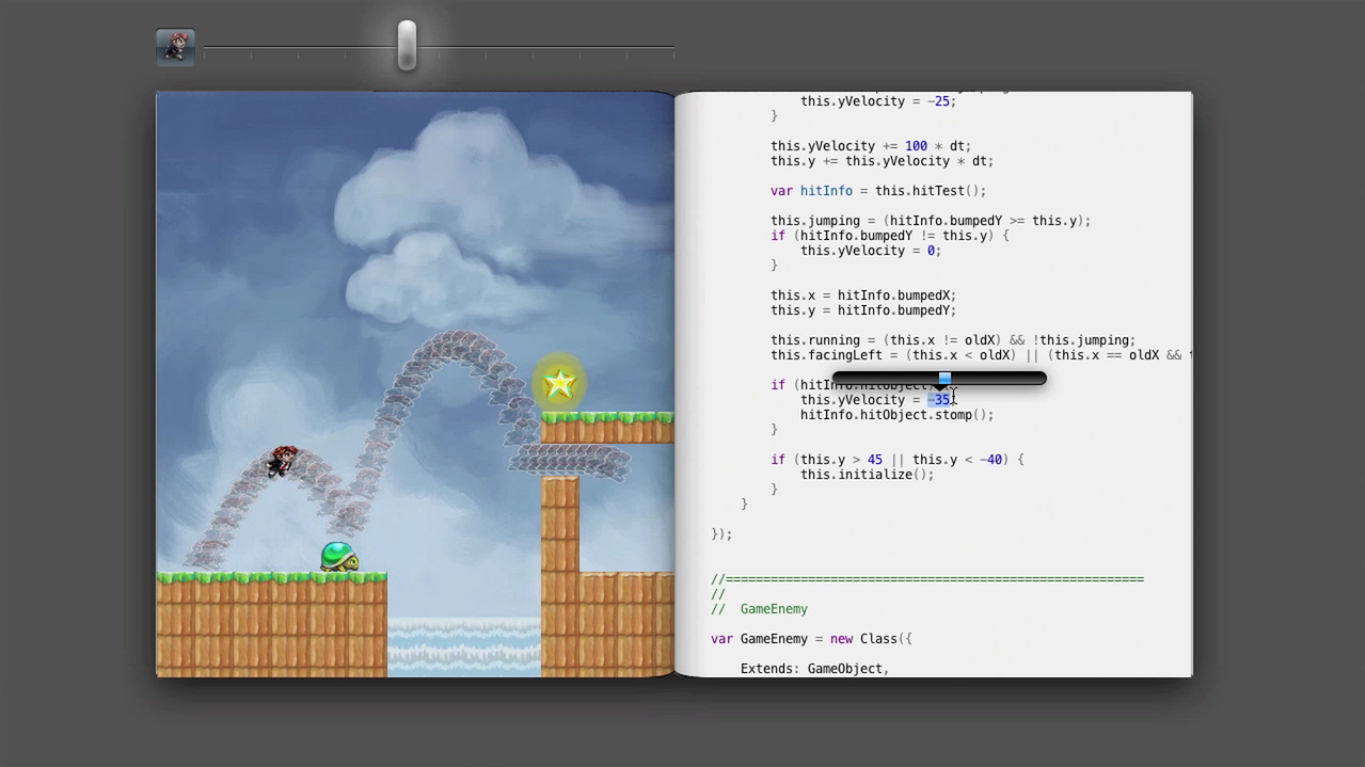
\includegraphics[width=1.0\textwidth]
		{./resources/figures/victor.png}

	\caption{
	An experimental graphical debugger, which allows for tweaking the
	recorded history of an application. 
	The image (taken from \cite{Victor2012}) depicts how
	the modification of a movement variable affects the recording.
	}
	\label{fig:victor}
\end{figure}


\section{Retroactive Aspects}
Retroactive aspects have been described by Salkeld et al. in various works 
\cite{Salkeld2011, Salkeld2015}. Their work settles in the area of 
aspect-oriented programming (AOP). 
%
AOP has some advantages over an object-oriented approach. For example, it 
can be cumbersome to realize crosscutting functionalities in object-oriented 
programming models. Examples of crosscutting functionalities are logging or 
authorization features which affect multiple objects. 
A typical object-oriented approach to handle crosscutting functionality in 
multiple objects, is to call the e.g. authorization methods within each object. 
%
In AOP, on the other hand, crosscutting functionalities can be implemented by
creating a new \emph{advice} for an additional authorization functionality. 
Next, it is configured which methods this advice applies to by specifying 
\emph{pointcuts}. The term \emph{weaving} refers to the process of producing 
an executable program with the source code and the aspects ``weaved in''.

The authors aim to analyze and manipulate recordings of a program's execution
post hoc (i.e. offline). For this analysis, they aim to extend an existing AOP 
language to support retroactive evaluation semantics.
Thus, the analysis code is written in the same environment as the program. 
The authors make the argument that this eases the creation and evaluation of 
analyses for average developers, whose expertise lies in the language in which 
the program was written, rather than in the usage of external tools.
Additionally, developers can use the familiar data types and functions from the 
program in the analysis code as well.
They refer to their primary goal as ``allow[ing] analysis code that is as close
as possible to the program's source code''. 
The term \emph{retroactive weaving} refers to the evaluation of retroactive 
aspects ``in relation to a previous execution'', meaning retroactive aspects 
are weaved into an existing trace.
\emph{Retroactive advice} describes the analysis, replay, and modification of 
former states.
%
From our understanding, retroactive aspects describe the interplay of 
retroactive advice and retroactive weaving used to conduct post hoc analysis of 
a recorded program execution.  

The authors recognize the issues of dealing with side effects in retroactive 
contexts: ``We are continuing to investigate the best approach for managing side 
effects. It is unclear how to rigorously permit intentional, safe side effects 
in retroactive advice: outputting results to the console or the file system 
should be permitted, for example [\dots]''. For the analysis code they propose 
to avoid side effects, for the application code they suggest the usage of an 
operator which enable the suppression or redirection of side effects from 
retroactive code.


\section{Retroactive Data Structures}
Retroactive data structures record the series of operations which have been
performed on them. It is then possible to retroactively insert, delete, or
update an operation in the past.
These data structures were first described by Demaine et al. \cite{Demaine2007},
with a focus on how to implement them efficiently. The authors highlight a broad 
number of applications which can benefit from using retroactive data structures. 
One example which they describe consists of weather stations which lose their 
connection to a central control system. Once they are reconnected, their data 
needs to be fed back into the system. Ideally this is done retroactively, as if 
the stations had been connected the whole time. 

The authors compare retroactive data structures to persistent data structures
and highlight the differences: In persistent data structures, several versions 
of an object are held and modifying the object is achieved by applying an 
operation on the latest version.
Retroactive data structures, on the other hand, focus on inserting, deleting, 
or updating operations which have been executed on an object \emph{in the past}, 
rather than on the latest version.

Any data structure can be retroactively manipulated by rolling a data structure 
back to a prior state, apply a change, and replaying forward again. However,
the authors argue that this often leads to inefficient manipulations with 
an expensive overhead.
They examine if arbitrary data structures can always be transformed to a 
data structure with support for \emph{efficient} retroactive manipulations
and prove that it is not possible to find such a generic transformation.
Realizing efficient retroaction depends on the use case: they describe a 
number of data structures which support efficient retroactive modifications 
(e.g. priority queues).
%
The authors furthermore distinguish between \emph{partially} and \emph{fully} 
retroactive data structures. Partially retroactive data structures enable the 
insertion and deletion of operations in the past. Queries are limited to the 
present time. 
Thus the outcome of retroactive operations can only be observed at the present 
time. Fully retroactive data structures additionally allow the specification of 
arbitrary times in the past when placing a query. The result of the query will 
then be as if it were executed at that time in the past.
The delimitations to our objectives are that we consider interactive event-sourced
applications, opposed to data structures with no behavior by themselves. 


\section{Version Control Systems}
Version control systems (VCSes) or source code management (SCM) tools, like Git 
or Subversion, provide capabilities for managing changes to files. Once a file 
is committed to the repository, a revision with this certain state is created.
If an altered version of the same file is committed to the system, a new revision 
is created. The current state of a file is derived from this series of commits. 
Additionally, VCS tools allow changes to be traced and revoked, as well as the 
creation of branches.
These branches contain the entire history of the repository up to a certain 
branching point. It is then possible to apply experimental changes in the branch, 
without affecting the main \mbox{(or ``master'')} branch. Results can be 
integrated back to the original branch by merging two branches.
Most modern VCSes, however, provide much more than this basic set of operations
(bisecting\footnote[1]{\href{https://git-scm.com/docs/git-bisect}{https://git-scm.com/docs/git-bisect}} 
the occurence of a bug, for example).
Many modern \mbox{VCSes} save just the delta (the ``diff'') to the previous 
revision; the current state is thus defined by this series of deltas.

VCSes are typically agnostic in terms of the files which they administer in a 
repository. They are decoupled tools which operate on a meta level -- they do not 
have any coupling with the files which they administer. Also the files in the 
repository do not have access to their own history, nor operations to manipulate 
their own history.
A commonality with the event sourcing domain is that the repository can possess 
append-only semantics as well and the series of commits defines the current 
state. Thus, retrospective operations, such as restoring and analyzing previous 
states, are possible. Additionaly, a typical VCS provides features which this 
thesis aims to examine in event-sourced systems: creating branches and merging 
changes back to a main branch.


\section{Time Travel Theory}
\label{sec:time-travel-theory}
Time travelling is a concept which describes the notion of moving forward and 
backward through time. The field has been subject to works of fiction, philosophy, 
and extensive scientific research.
There are many parallels to the topic of retroaction in event-sourced systems: 
The event log can be considered a timeline and retroactive changes can be 
considered time travel. Furthermore, in time travel theory, a small change in 
the timeline can have enormous, unforeseeable changes as a consequence as well. 
%
An extensive summary of logical and philosophical questions on the topic was 
compiled by Smith \cite{Smith2016}. 
%
A number of interesting hypothetical questions (e.g. ``Where are the Time 
Travellers?'') are discussed there as well.

Time travel theory can provide helpful insights on issues of retrocausality and 
causality violations which might occur. Causality violations in time travel 
theory occur when we observe an effect before its cause. One such issue concerns 
the emergence of temporal paradoxes, which can lead to an event log that is in 
contradiction to itself.
Consider the \emph{grandfather paradox}: one goes back in time to a point before 
one's own father was conceived and eliminates one's grandfather. This leads to a 
paradox: once the grandfather is dead, one could never have been born and never 
have travelled back in time to murder one's own grandfather. This is a logical 
paradox, each scenario contains its own exclusion. 
Transferred to an event-sourced system, a comparable scenario is an object which 
removes its producer from the log at a point before it was created.

But issues of retrocausality do not always require family members to die. Another 
problem of retrocausality concerns \emph{causal loops} which emerge when one event 
is cause for another event, which is a retroactive cause for the first event. Or 
as the physicist Michael Rea puts it: ``a causal loop is a causal chain in which 
at least one of the events in the chain lies in its own history'' \cite{Rea2014}.
%
Without further considerations, it cannot be determined what originally triggered 
the event and causal loops can be responsible for loops in which ``things come 
from nowhere'' \cite{Smith2016}.
%
Various examples of causal loops have been constructed by philosophers, physicists, 
and fiction authors. These examples often have a similar pattern and the presumption 
of a single timeline (often referred to as a ``closed timelike curve''). 
One such example is a time traveller who travels back with the copy of a mathematical 
proof. The traveller reveals this proof to the mathematician who made this very proof,
at a time before he did it. Thus the information seems to come from nowhere.
%
When computed, causal loops can create infinite loops. They can also break the 
traceability of a system, since it is not always clearly determinable how a system 
reached its current state.
We examine these issues of causalities in retroactive systems in further 
detail in Chapter \ref{chp:concept}.

A number of theories postulate possibilities to avoid paradoxes. One such theory 
concerns \emph{parallel universes}. Here, each time travelling action yields a new, 
parallel, universe. If the grandson eliminates his grandfather in this new, parallel, 
universe, his action will not impact his conception in the original universe. 
The elimination happened on a different timeline, thus there is no paradox.
This idea is also commonly described as ``many-worlds interpretation''.
Another possibility is the \emph{self-consistency principle} \cite[p.607]{Frolov1998}, 
which was developed by Igor Novikov to solve the problem of time travel paradoxes.
It postulates that actions which would lead to paradoxes simply cannot be 
executed -- similar to the laws of physics which restrain our influence on 
the real world.
In works of fiction this self-consistency is sometimes depicted as a restriction
of the free will (one just cannot act in this way) or by creative avoidances, such
as that one's grandfather was not actually the biological grandfather.

Whether time travel is possible remains disputed. As we view it, the scientific 
and philosophical consensus seems to be that time travel is assessed as unlikely. 
The argumentation often follows the lead that time travel raises a number of issues 
which cannot be explained with current scientific or philosophical understandings.


\section{Other Related Domains}
In the area of discrete-event simulation (DES), a system is modelled as a sequence 
of discrete events. Here, events are defined as ``\emph{instants in time when a 
state-change occurs}'' \cite{Robinson2004}. 
Such a simulation is executed by tracing the path from one event to its consecutive 
event(s). State is represented as discrete events over time with the current state 
being derived from this series of events. This concept has a number of parallels 
to the ideas behind event sourcing.
In fact, there are so many commonalities between the two research domains that 
it is possible to combine them. In a work by Erb and Kargl \cite{Erb2014}, both 
approaches are compared; they also describe a hybrid architecture.

There are a number of further research domains and technological fields with parallels 
to retroaction in event-sourced systems. Database management systems often possess 
transaction logs and rollback methods for fault or crash recovery \cite{Ramakrishnan2000}. 
Journaling file systems, such as ext4 or JFS, record the state mutating operation for 
crash or fault recovery.
Message logging and checkpointing is another concept used in distributed systems for 
failure or crash recovery.
Besides the already described retroactive data structures, there are more data structures 
with history support. The concept of unlimited undo or backtracking \cite{Apostolico1994}
is such an example.
The blockchain technology \cite{Swan2015} used in the Bitcoin cryptocurrency (and many 
other applications) has parallels to event-sourced systems as well. The blockchain 
utilizes cryptography to achieve an immutable property for blocks. In conjunction with 
the append-only behavior of the blockchain, this can be beneficial for scalability and 
traceability (audit log). 
%
A multitude of NoSQL databases view modifications of documents as incremental state 
changes, which are committed to an append-only data storage. CouchDB is such an example 
\cite{Anderson2010}.


\section{Summary}
In this section, we described a number of related research domains and technological 
fields. We highlighted that a lot of the ideas behind event sourcing and retroaction 
can be found in other areas as well, mostly under a different terminology.
%
Most systems, however, use a post hoc analysis approach, in which the analysis tool 
is in a separate environment, tool, or programming model. When the history of a 
system is utilized, this is mostly done by applying only passive retrospection, 
without retroactively altering the application's history.

The objective of this thesis is to examine an integrated system, where an application 
may modify and interact with its history in a single environment. To the best of our 
knowledge, the idea of using an event-sourced architecture to enable retroactive 
computing features has not yet been researched, nor examined within a prototypical 
implementation.
